%\documentclass[mat1]{fmfdelo}
% \documentclass[fin1]{fmfdelo}
% \documentclass[isrm1]{fmfdelo}
 \documentclass[mat2]{fmfdelo}
% \documentclass[fin2]{fmfdelo}
% \documentclass[isrm2]{fmfdelo}

% naslednje ukaze ustrezno napolnite
\avtor{Ime Priimek}

\naslov{Naslov dela}
\title{Angleški prevod slovenskega naslova dela}

% navedite ime mentorja s polnim nazivom: doc.~dr.~Ime Priimek,
% izr.~prof.~dr.~Ime Priimek, prof.~dr.~Ime Priimek
% uporabite le tisti ukaz/ukaze, ki je/so za vas ustrezni
\mentor{}
% \mentorica{}
% \somentor{}
% \somentorica{}
% \mentorja{}{}
% \mentorici{}{}

\letnica{} % leto diplome

%  V povzetku na kratko opišite vsebinske rezultate dela. Sem ne sodi razlaga organizacije dela --
%  v katerem poglavju/razdelku je kaj, pač pa le opis vsebine.
\povzetek{}

%  Prevod slovenskega povzetka v angleščino.
\abstract{}

% navedite vsaj eno klasifikacijsko oznako --
% dostopne so na www.ams.org/mathscinet/msc/msc2020.html
\klasifikacija{}
\kljucnebesede{} % navedite nekaj ključnih pojmov, ki nastopajo v delu
\keywords{} % angleški prevod ključnih besed

\zapisiMetaPodatke  % poskrbi za metapodatke in veljaven PDF/A-1b standard

% aktivirajte pakete, ki jih potrebujete
\usepackage{tikz}
\usepackage{graphicx}
\usetikzlibrary{arrows,matrix,positioning, arrows.meta}
\usepackage{scalerel}
\usepackage[shortlabels]{enumitem}


% za številske množice uporabite naslednje simbole
\newcommand{\R}{\mathbb R}
\newcommand{\N}{\mathbb N}
\newcommand{\Z}{\mathbb Z}
\newcommand{\C}{\mathbb C}
\newcommand{\Q}{\mathbb Q}

% matematične operatorje deklarirajte kot take, da jih bo Latex pravilno stavil
% \DeclareMathOperator{\conv}{conv}
\DeclareMathOperator{\interior}{int}

% vstavite svoje definicije ...
\newcommand{\dashedTri}{%
        \begin{tikzpicture}

\tikzset{vertex/.style = {shape=circle, fill=black,draw,minimum size=3pt, inner sep=0pt}}
\tikzset{edge/.style = {->,> = latex'}}
\tikzset{interval/.style = {<->,> = {Bracket[length=0.8mm, width=4mm]}, line width = 0.8pt}}
% vertices
\node[vertex] (1) at  (0, 0) {};
\node[vertex] (2) at  (0.8, 0) {};
\node[vertex] (3) at  (1.6, 0) {};
%edges
\draw[edge, dashed] (1) to[bend left=12] (2);
\draw[edge, dashed] (2) to[bend left=12] (3);
\draw[edge, dashed] (3) to[bend left=10] (1);
\end{tikzpicture}%
    }
    
    \makeatletter
  \begingroup
    \setbox\@tempboxa=\hbox{$\subset$}
    \@tempdima=\dp\@tempboxa
    \newbox\@sarabox
    \global\setbox\@sarabox=\hbox{%
      \begin{tikzpicture} [baseline=0pt, line cap=round]
        \node (subset) at (0,-\@tempdima) [above left, inner sep=0pt, outer sep=0pt] {$\subset$};
        \begin{pgfinterruptboundingbox}
          \draw (-2.5pt,6.2pt) edge [->] +(1.5pt,0pt);
       \end{pgfinterruptboundingbox}
      \end{tikzpicture}%
    }
    \global\ht\@sarabox=\ht\@tempboxa
  \endgroup
  \newcommand*\sara{\mathrel{\scalerel*{\usebox\@sarabox}{\subset}}}
\makeatother

%  \newcommand{}{}


\begin{document}

\section{Uvod}
Napišite kratek zgodovinski in matematični uvod.  Pojasnite motivacijo za problem, kje
nastopa, kje vse je bil obravnavan. Na koncu opišite tudi organizacijo dela -- kaj je v
katerem razdelku.

\section{definicije in formulacija izreka}
Naj bo $I\subseteq \R$ povezana podmnožica realnih števil. Takim množicam domo rekli intervali. Interval ne rabi biti zaprt ali omejen in lahko v nekaterih primerih predstavlja kar celotno množico realnih števil. Naj bo $f:I \to I$ zvezna funkcija, ki slika interval $I$ nazaj vase. Ker funkcija $f$ slika interval $I$ nazaj vase, si jo lahko predstavljamo kot diskreten dinamični sistem. S $f^n$ bomo označevali kompozitum:
$$f^n = \underbrace{f \circ f \circ \cdots \circ f}_{n \text{ ponovitev } f},$$
kjer $f^0$ predstavlja identično funkcijo. S pomočjo iteracij funkcije $f$ definiramo zaporedje s splošnim členom $x_n = f^n(x_0)$.

\begin{figure}[h]
  \centering
  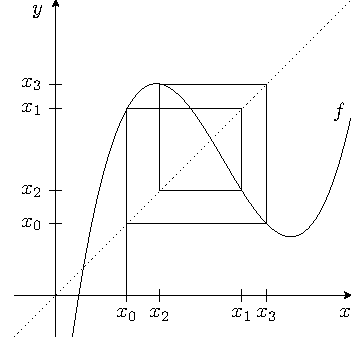
\includegraphics[]{images/iteracije_f.pdf}
% \caption[caption za v kazalo]{Dolg caption pod sliko}
  \caption[Primer vektorske slike.]{Slika prikazuje, iteracije funkcije $f$.}
  \label{fig:Iteracije}
\end{figure}

V takem dinamičnem sistemu ena iteracija funkcije predstavlja en diskreten korak v času, točka $x_0 \in I$ pa začetni položaj točke v sistemu. Množici, ki vsebuje vse člene zaporedja bomo rekli $f$-orbita točke $x_0$ ali samo orbita točke $x_0$. Z matematičnimi simboli jo lahko zapišemo tako:
$$\{ \mathcal{O} := f^m(x_0) ; m \in \N \}.$$
Izrek Šarkovskega preučuje take točke $x_0 \in I$, ki se po nekaj iteracijah s funkcijo $f$ slikajo nazaj vase. Takim točkam rečemo periodične točke. Perioda točke $x_0$ je najmanjše tako naravno število $n$, za katerega je $f^n(x_0) = x_0$. Ekvivalentno lahko sklepamo, da je orbita periodične točke $x_0$ končna množica, število različnih elementov v orbiti pa je enako periodi točke $x_0$. Fiksna točka je periodična točka s periodo 1, torej taka točka $x_0$, za katero je $f(x_0) = x_0$. Če obstaja periodična točka s periodo $m$, rečemo tudi, da ima funkcija $f$ periodo $m$.

Pri danem dinamičnem sistemu se lahko vprašamo, katere periode lahko ima funkcija. Šarkovski si je postavil prav to vprašanje in prišel do ureditve množice naravnih števil, ki pove, katere periode lahko ima funkcija.

\subsection{Izrek Šarkovskega}

\begin{definicija}
Množico naravnih števil lahko uredimo na naslednji način:
$$3 \triangleleft 5 \triangleleft 7 \triangleleft \cdots \triangleleft 2\cdot 3 \triangleleft 2\cdot 5 \triangleleft 2\cdot 7 \triangleleft \cdots \triangleleft 2^2\cdot 3 \triangleleft 2^2\cdot 5 \triangleleft 2^2\cdot 7 \triangleleft \cdots \triangleleft 2^3 \triangleleft 2^2 \triangleleft 2 \triangleleft 1.$$
Ureditev, imenujemo jo ureditev Šarkovskega, določa relacijo $\triangleleft$. Naravni števili $m$ in $n$ sta v relaciji $m\triangleleft n$ natanko tedaj, ko $m$ leži levo od $n$ ali je $m=n$. Prepričajmo se, da je relacija $\triangleleft$ relacija linearne urejenosti. Najprej opazimo, da je ureditev sestavljena tako, da najprej naštejemo liha števila večja od 1, nato dodamo ta števila po vrsti pomnožena z 2. Sledijo liha števila večja od 1 pomnožena z $2^2$ itn. Na koncu so zapisane potence števila 2 v padajočem vrstnem redu. Zaradi vrstnega reda števil pomislimo, da lahko vsako naravno število zapišemo kot produkt potence števila 2 in nekega lihega števila. To pomeni, da lahko poljubni naravni števili $m$ in $n$ zapišemo na naslednji način: $m= 2^k(2m_1 +1)$ in $n= 2^l(2n_1 +1)$, kjer so števila $m_1, n_1, k, l \in \N_0$. Števili sta v relaciji $m \triangleleft n$, če je:
\begin{enumerate}
\item $k<l$ in $m_1 \neq 1$ in $n_1 \neq 1$ ali
\item $k=l$ in $m_1 \leq n_1$ ali
\item $k>l$ in $m_1 = n_1$ ali
\item $k>0$ in $l =0$.
\end{enumerate}
Lahko je preveriti, da je tako definirana relacija refleksivna, antisimetrična, tranzitivna in sovisna.
S pomočjo zapisa relacije se enostavno prepričamo v naslednjo pomembno lastnost relacije:
$$\text{za } m, n \in \N: m \triangleleft n \Leftrightarrow 2m \triangleleft 2n.$$

\end{definicija}



\begin{izrek}[The Sharkovsky forcing theorem]\label{izr:forcing}
Če ima $f : I \to I$ točko periode $m$ in velja $ m \triangleleft l$, potem obstaja tudi točka periode $l$.
\end{izrek}
Izrek pove, da je množica period zvezne funkcije na intervalu $I$ rep ureditve Šarkovskega. Rep ureditve Šarkovskega je taka množica $\mathcal{T} \subset \N$, za katero je $m \triangleleft n$ za  vsaki naravni števili $m \notin \mathcal{T}$ in $n \in \mathcal{T}$. Obstajajo trije različni tipi repov:  Za neko naravno število $m$ je rep množica $\{n \in \N; m \triangleleft n\}$, množica $\{\dots, 16, 8, 4, 2, 1\}$ vseh potenc števila 2 in $\emptyset$.
Naslednji izrek je neke vrste obrat zgornjega izreka.

\begin{izrek}[The Sharkovsky realization theorem]\label{izr:realization}
Za vsak rep $\mathcal{T}$ v zaporedju Šarkovskega obstaja taka funkcija, katere množica period je enaka $\mathcal{T}$.
\end{izrek}

Izrek Šarkovskega je unija izreka~\ref{izr:forcing} in izreka~\ref{izr:realization}. Podmnožica naravnih števil je množica period zvezne funkcije $f:I \to I$, če in samo če je množica rep ureditve Šarkovskega. Nasledja poglavja so namenjena pripravi na dokaz izreka~\ref{izr:forcing}, v poglavju pa je predstavljen dokaz.
\section{Intervali, relacija pokritja in cikli}
Vsi dokazi izreka Šarkovskega so si podobni po tem, da so elementarni. Ne glede na to, kako zvito se lotimo dokaza, je ključnega pomena lastnost zveznih funkcij, ki zagotavlja obstoj ničle funkcije. To je izrek o vmesni vrednosti.

\begin{izrek}[izrek o vmesni vrednosti]\label{izr:iovv}
Funkcija $f$, ki je zvezna na intervalu $[a, b]$ in je na krajiščih intervala različno predznačena, torej velja neenačba $f(a)\cdot f(b) < 0$, ima vsaj v eni točki tega intervala vrednost 0.
\end{izrek}

\begin{figure}[h]
  \centering
  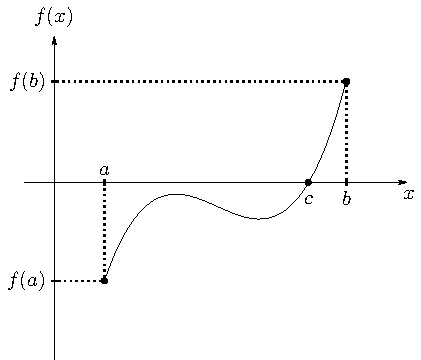
\includegraphics[]{images/intermediate.pdf}
% \caption[caption za v kazalo]{Dolg caption pod sliko}
  \caption[Primer vektorske slike.]{Slika prikazuje, kako poiščemo interval $K$.}
  \label{fig:bezje}
\end{figure}

\begin{proof}
Naj bo funkcija $f:[a, b] \to [a, b]$ zvezna in naj bo $f(a)\cdot f(b) < 0$. Brez izgube splošnosti lahko predpostavimo, da je $f(a) < 0 < f(b)$. Ničlo funkcije $f$ bomo iskali s pomočjo deljenja intervalov oziroma z bisekcijo. Izračunamo razpolovišče $p_0=\frac{a+b}{2}$ intervala $[a, b]$.Če je $f(p)=0$, smo ničlo že našli, sicer razmišljamo tako: če je $f(p_0) >0$, označimo $[a_1, b_1] =  [a, p_0]$, sicer označimo $[a_1, b_1] =  [p_0, b]$. Nato izračunamo razpolovišče $p_1$ intervala $[a_1, b_1]$. Če je $f(p)=0$ postopek ustavimo, saj smo ničlo našlio, v nasprotnem primeru pogledamo predznak $f(p_1)$. Če je $f(p_1) >0$, označimo $[a_2, b_2] =  [a_1, p_1]$, sicer označimo $[a_2, b_2] =  [p_1, b_1]$. Postopek nadaljujemo dokler ne najdemo ničle $p_i$ funkcije $f$. Če ničle ne najdemo, dobimo neskončno zaporedje vloženih intervalov 
$$ [a, b] \supset [a_1, b_1] \supset [a_2, b_2] \supset \cdots$$
Lahko se prepričamo, da je $b_n - a_n = \frac{b-a}{2^n}$ in $f(a_n)<0<f(b_n)$ za vsak $n\in \N$. Števila $a_n$ tvorijo naraščajoče zaporedje, števila $b_n$ pa padajoče zaporedje.  Limiti $\lim\limits_{n \to \infty} a_n$ in $\lim\limits_{n \to \infty} b_n$ sta enaki, saj je 
$\lim\limits_{n \to \infty} b_n - \lim\limits_{n \to \infty} a_n = \lim\limits_{n \to \infty} (b_n - a_n) =0$. Označimo $c = \lim\limits_{n \to \infty} a_n = \lim\limits_{n \to \infty} b_n$. Potem je 
$\bigcap\limits_{n=1}^{\infty} [a_n, b_n] = \{c\}$. 
Ker je funkcija zvezna je 
$\lim\limits_{n \to \infty} f(a_n) = f(\lim\limits_{n \to \infty} a_n) = f(c)$
in 
$\lim\limits_{n \to \infty} f(b_n) = f(\lim\limits_{n \to \infty} b_n) = f(c)$.
Za vsako naravno število $n$ velja $f(a_n) <0$, zato je $f(c) \leq 0$. Podobn je $f(b_n) > 0$ za vsako naravno število $n$, iz česar sklepamo, da je $f(c) \geq 0$. Torej je $f(c) = 0$, kar zaključi dokaz.
\end{proof}

\begin{definicija}\label{def:pokritja}
Pravimo, da interval $I$ pokrije interval $J$, če je $J \subseteq f(I)$. Relacijo zapišemo kot $I \rightarrow J$. Kadar velja $f(I) =J$, zapišemo $I \rightarrowtail J$.
\end{definicija}

S pomočjo izreka o vmesni vrednosti in poznavanja, kako se intervali slikajo s funkcijo $f$ lahko izvemo, ali obstajajo periodične točke. Kako lahko potrdimo obstoj periodičnih točk, nam povejo naslednje leme.

\begin{lema}\label{lem:1zanka}
Če je $[a, b] \to [a, b]$, potem ima funkcija $f$ fiksno točko na intervalu $[a, b]$.
\end{lema}
\begin{proof}
Interval $[a, b]$ je podmnožica slike $f([a, b])$, zato obstajata taki točki $a_1, b_1 \in [a, b]$, da je $f(a_1)=a$ in $f(b_1)=b$. Definiramo funkcijo $g(x) = f(x) - x$. Zaradi neenakosti 
$$b_1-f(b_1) =b_1-b<0<a_1-a=a_1-f(b_1),$$
je zvezna funkcija $g$ na krajiščih intervala $[a, b]$ različno predznačena. Po izreku~\ref{izr:iovv} obstaja točka $c \in [a, b]$, pri kateri je $g(c)=0$, torej je $f(c) = c$.
\end{proof}


\begin{lema}\label{lem:zanka}
Če so intervali $I_0, \dots, I_{n-1}$ zaprti omejeni intervali za katere veljajo naslednje relacije pokritosti: $I_0 \to \dots \to I_{n-1} \to I_0$, potem obstaja taka točka $x$, za katero je $f^{i}(x) \in J_i$ za $0 \leq i < n$ in $f^n(x)=x$. Pravimo, da točka $x$ sledi zanki.
\end{lema}

\begin{proof}
Pišemo $I \rightarrowtail J$, če je $f(I) = J$. Če velja relacija pokritosti $I \to J$, obstaja tak interval $K \subset I$, da je $K \rightarrowtail J$.
\begin{figure}[h]
  \centering
  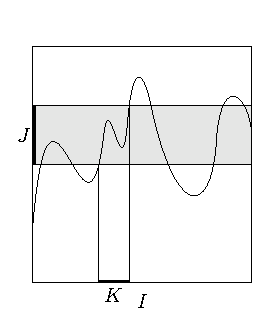
\includegraphics[]{images/bezje.pdf}
% \caption[caption za v kazalo]{Dolg caption pod sliko}
  \caption[Primer vektorske slike.]{Slika prikazuje, kako poiščemo interval $K$.}
  \label{fig:bezje}
\end{figure}
Interval $K$ poiščemo tako, da iz preseka funkcije $f$ s pravokotnikom $I \times J$ izberemo povezan del grafa, ki povezuje spodni in zgornji del pravokotnika. Tak del zagotovo obstaja, saj je $J \subset f(I)$. Projekcijo tega dela na interval $I$ označimo s $K$. Torej, obstaja tak interval $K_{n-1} \subset J_{n-1}$, da je $K_{n-1} \rightarrowtail J_0$. Velja relacija pokritosti $J_{n-2} \to K_{n-1}$, zato obstaja tak interval $K_{n-2} \subset J_{n-2}$, da je $K_{n-2} \rightarrowtail K_{n-1}$. S postopkom nadaljujemo in dobimo naslednje relacije:
$$K_0 \rightarrowtail K_1 \rightarrowtail \cdots \rightarrowtail K_{n-1} \rightarrowtail J_0.$$
Za vsako točko $x \in K_0$ in za vsak $i \in [0, n)$ velja $f^i(x) \in K_i \subset J_i$ in $f^n(x) \in J_0$. Ker je $K_0 \subset J_0 = f^n(K_0)$, lahko s pomočjo leme XXX sklepamo, da ima $f^n$ fiksno točko na intervalu $K_0$.
\end{proof}

Obravnavajmo zvezno funkcijo $f(x) = x^2$ na intervalu $[0, 1]$. Na tem intervalu sta samo dve točki, ki sledita $2$-zanki. To sta točki $0$ in $1$, ki imata periodo 1.
Zato se z obstojem periodičnih točk pa se za enkrat še ne moremo zadovoljiti. Radi bi vedeli, da je perioda točke enaka dolžini zanke in ne kakšen pravi delitelj dolžine.

\begin{definicija}\label{def:element}
Zanka intervalov $I_0 \to \cdots \to I_{n-1} \to I_0$ je elementarna, če ima vsaka točka, ki sledi zanki, periodo $n$.
\end{definicija}

\begin{posledica}
Vsaka elementarna zanka intervalov $I_0 \to \dots \to I_{n-1} \to I_0$ vsebuje točko $a$, ki sledi zanki in ima periodo $n$.
\end{posledica}

Zaradi zgornje posledice bi bilo dobro, če bi poznali kakšen dober kriterij za prepoznavanje elementarnih zank. Najlažji kriterij je število intervalov v zanki. Če nastopa samo en interval, dobimo $I_0 \to I_0$. To je elementarna zanka. Naslednja lema poda še en kriterij Za prepoznavanje elementarnih zank:

\begin{lema}\label{lem:element}
Zanka intervalov $I_0 \to \cdots \to I_{n-1} \to I_0$ je elementarna, če ji ne sledi nobena robna točka in je notranjost intervala $\interior(I_0)$ disjunktna z intervali $I_1, \dots, I_{n-1}$. Torej, $\interior(I_0) \cap \bigcup_{i=1}^{n-1}I_i = \emptyset$.
\end{lema}
\begin{proof}
Točka $x_0$, ki sledi zanki ne more biti robna točka intervala $I_0$. Torej je $x_0 \in \interior(I_0)$. Za vsak $i=1, \dots, n-1$ je $x_0 \neq f^i(x_0)$, saj je $f^i(x_0) \in I_i$, intervala $I_0$ in $I_i$ pa sta disjunktna. Ker točka $x_0$ sledi zanki je $f^n(x_0)=x_0$. Točka $x_0$ ima periodo $n$.
\end{proof}

\section{Primeri}%################ POGLAVJE S PRIMERI
V tem poglavju si bomo zaradi lažjega razumevanja pogledali nekaj posebnih primerov. Najprej si bomo pogledali najbolj znan poseben primer izreka Šarkovskega. V naslednjih dveh primerih bomo postopek iz prvega primera razširili na daljše cikle. V zadnjem primeru bomo nakazali indukcijski korak, ki ga bomo uporabili v dokazu izreka.

\begin{primer}[3-cikel]\label{primer1}
Perioda 3 implicira obstoj vseh ostalih period. Točka lahko tvori $3$-cikel na dva različna načina, ki sta v resnici zrcalna podoba drug drugega. Slika prikazuje oba primera. 
\begin{figure}[h]
  \centering
  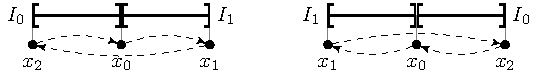
\includegraphics{images/tricikel.pdf}
% \caption[caption za v kazalo]{Dolg caption pod sliko}
  \caption[Primer vektorske slike.]{Zrcalna podoba ciklov}
  \label{fig:3cikla}
\end{figure}
Črtkane puščice nakazujejo, kam se s funkcijo $f$ slikajo točke. Velja: 
$$x_1 = f(x_0), x_2 = f(x_1) \text{ in } x_0 = f(x_2).$$
V obeh primerih smo z $I_1$ označili $\mathcal{O}$-interval s krajišči $x_0$ in $x_1$, z $I_0$ pa $\mathcal{O}$-interval s krajišči $x_0$ in $x_2$. Krajišči intervala $I_1$ se slikata v skrajno levo in skrajno desno točko cikla, zato imamo $\mathcal{O}$-vsiljeni pokritji $I_1 \to I_1$ in $I_1 \to I_0$. Krajišči intervala $I_0$ se slikata v krajišči intervala $I_1$, zato je tudi pokritje $I_0 \to I_1$ $\mathcal{O}$-vsiljeno. Ugotovljena pokritja lahko strnemo v diagram $\sara I_1 \leftrightarrows I_0$. Iz relacije pokritosti $I_1 \to I_1$ in leme~\ref{lem:1zanka} sklepamo, da interval $I_1$ vsebuje negibno točko. Krajišči intervala $I_1$ ne morejo slediti zanki $I_1 \to I_0 \to I_1$, saj sta periodični točki s periodo 3. Točke, ki sledijo zanki, pa imajo periodo 1 ali 2. Ker je notranjost intervala $I_0$ disjunktna z intervalom $I_1$, lahko s pomočjo leme~\ref{lem:element} sklepamo, da je zanka 
$$I_0 \to \overbrace{I_1 \to I_1 \to \cdots \to I_1}^{l-1 \text{ ponovitev intervala } I_0} \to I_0$$
elementarna za $l > 3$.
\end{primer}


\begin{primer}[7-cikel] \label{primer2}
Sedaj bomo obravnavali 7-cikel $\mathcal{O}$ in $\mathcal{O}$-intervale prikazane na sliki.
\begin{figure}[h]
  \centering
  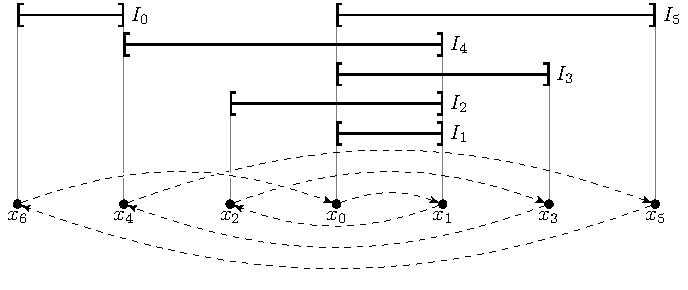
\includegraphics{images/sedemcikel.pdf}
% \caption[caption za v kazalo]{Dolg caption pod sliko}
  \caption[Primer vektorske slike.]{Primer 7-cikla.}
  \label{fig:7cikel}
\end{figure}
 Podobno kot pri prejšnjem primeru označimo $x_i = f^i(x_0)$ in $I_1 = [x_0, x_1]$ in tako naprej, kot prikazuje slika. Za to izbiro intervalov dobimo naslednje $\mathcal{O}$-vsiljene relacije pokritosti:
\begin{enumerate}
\item $I_1 \to I_1$
\item $I_1 \to I_2 \to I_3 \to I_4 \to I_5 \to I_0$
\item $I_0 \to I_1$, $I_0 \to I_3$ in $I_0 \to I_5$
\end{enumerate}
Zgornje relacije pokritosti lahko prikažemo z diagramom, kot ga prikazuje slika:
\begin{figure}[h]
  \centering
  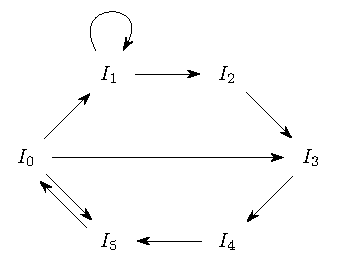
\includegraphics{images/graph6.pdf}
% \caption[caption za v kazalo]{Dolg caption pod sliko}
  \caption[Primer vektorske slike.]{diagram}
  \label{fig:6kotnik}
\end{figure}
Iz grafa preberemo naslednje zanke.
\begin{enumerate}
\item $I_1 \to I_1$
\item $I_0 \to I_5 \to I_1$
\item $I_0 \to I_3 \to I_4 \to I_5 \to I_0$
\item $I_0 \to I_1 \to I_2 \to I_3 \to I_4 \to I_5 \to I_0$
\item $I_0 \to \underbrace{I_1 \to I_1 \to \cdots  \to I_1}_{l \text{ ponovitev intervala } I_1} \to I_2 \to I_3 \to I_4 \to I_5 \to I_0$, kjer je $l\geq 3$.
\end{enumerate}
Zanka $I_1 \to I_1$ je elementarna, saj je elementarna vsaka zanka dolžine 1. Pri ostalih zankah pa lahko ugotovimo, da za vsak $j \in \{1, 2, \dots, 5\}$ velja $\interior(I_0) \cap I_j = \emptyset$. Nobena robna točka intervala $I_0$ ne more slediti zanki, saj je perioda robnih točk 7, perioda točke ki sledi intervalu pa različna od 7. S tem razmislekom so izpolnjeni pogoji leme~\ref{lem:element}, zato lahko sklepamo, da so zanke elementarne. Torej lahko na podlagi prisotnosti tega cikla sklepamo, da so prisotne vse periode $l$, za katere je $l \triangleleft 7$
\end{primer}

\begin{primer}[9-cikel] \label{primer3}
Slika prikazuje 9-cikel $\mathcal{O}$ neke funkcije, za katerega smo izbrali 6 $\mathcal{O}$-intervalov $I_0, I_1, \dots, I_5$, za katere je $\interior(I_0) \cap I_j = \emptyset$ za $0\leq j \leq 5$
\begin{figure}[h]
  \centering
  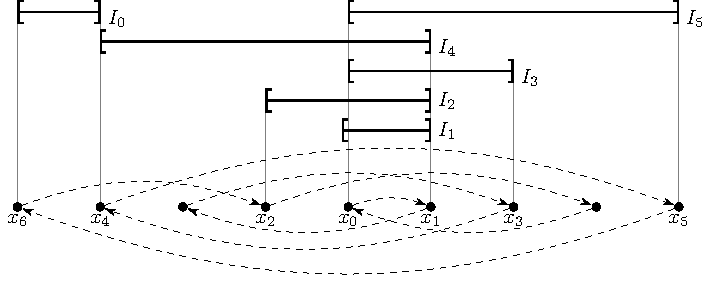
\includegraphics{images/devetcikel.pdf}
% \caption[caption za v kazalo]{Dolg caption pod sliko}
  \caption[Primer vektorske slike.]{Primer 9-cikla.}
  \label{fig:9cikel}
\end{figure}

\begin{figure}[h]
  \centering
  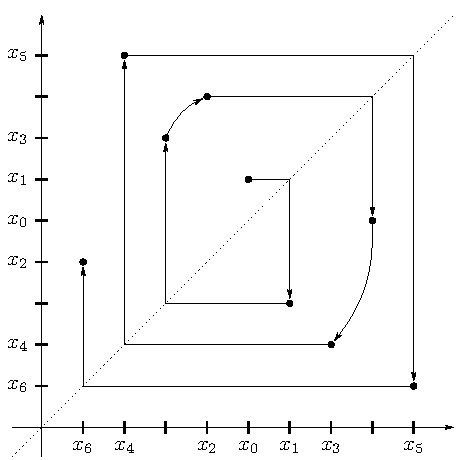
\includegraphics{images/spiral.pdf}
% \caption[caption za v kazalo]{Dolg caption pod sliko}
  \caption[Primer vektorske slike.]{Primer 9-cikla.}
  \label{fig:spiral}
\end{figure}


\end{primer}

\begin{primer}[6-cikel] \label{primer4}
Obravnavali bomo 6-cikel, ki je na sliki~\ref{fig:6cikel}. Bistveno pri tem primeu je, da se tri točke na levi strani slikajo v tri točke na desni in obratno. Torej, tri točke na desni tvorijo 3-cikel
\tikz{
\tikzset{vertex/.style = {shape=circle, fill=black,draw,minimum size=3pt, inner sep=0pt}}
\tikzset{edge/.style = {->,> = latex'}}
	\node [vertex](1) at  (0, 0) {};
	\node[vertex] (2) at  (0.8, 0) {};
	\node[vertex] (3) at  (1.6, 0) {};
	\draw[edge, dashed] (1) to[bend left=20] (2);
	\draw[edge, dashed] (2) to[bend left=20] (3);
	\draw[edge, dashed] (3) to[bend left=15] (1);
}
 za funkcijo $f^2$. Podobno kot v primeru~\ref{primer1} lahko določimo intervala $I_0$ in $I_1$ ter opazujemo relacije pokritja $I_1 \xrightarrow{f^2} I_1$, $I_1 \xrightarrow{f^2} I_0$ in $I_0 \xrightarrow{f^2} I_1$ za intervala $I_0$ in $I_1$, ki sta prikazana na sliki~\ref{fig:6cikel}. Enako kot prej lahko zaključimo, da ima funkcije $f^2$ elementarne zanke vseh dolžin in zato je vsako naravno število $l \in N$ perioda funkcije $f^2$. Za funkcijo $f$ določimo še dva intervala. Interval $I_0'$ naj bo najkrajši $\mathcal{O}$-interval, ki vsebuje točke iz množice $f(I_0 \cup \mathcal{O})$, interval $I_1'$ pa naj bo najkrajši $\mathcal{O}$-interval, ki vsebuje točke iz množice $f(I_1 \cup \mathcal{O})$. Sedaj bomo prikazali rekurzivno metodo, ki jo bomo uporabili kasneje v dokazu. Pokazali bomo, kako lahko s pomočjo elementarne $k$-zanke za funkcijo $f^2$ poiščemo elementarno $2k$-zanko za funkcijo $f$. V primeru, ki ga obravnavamo, bo to pomenilo, da je vsako sodo naravno število perioda funkcije $f$.
Poglejmo si elementarno $k$-zanko za funkcijo $f^2$, v kateri nastopajo relacije pokritja 
$I_1 \xrightarrow{f^2} I_1$, $I_1 \xrightarrow{f^2} I_0$ in $I_0 \xrightarrow{f^2} I_1$. Vsak zapis $I_1 \xrightarrow{f^2}$ v zanki lahko zamenjamo z $I_1 \xrightarrow{f} I_1'  \xrightarrow{f}$, vsak zapis $I_0 \xrightarrow{f^2} $ pa z $I_0 \xrightarrow{f} I_0'  \xrightarrow{f}$. S to spremembo dobimo $2k$-zanko za funkcijo $f$, ki ni samo dvakrat ponovljena $k$-zanka. Prepričajmo se, da je $2k$-zanka elementarna. Denimo, da točka $p$ sledi $2k$-zanki za funkcijo $f$. Pokazati moramo, da ima periodo $2k$ za funkcijo $f$. Opazimo, da točka $p$ sledi prvotni $k$-zanki za funkcijo $f^2$ in ima zato periodo $k$ za funkcijo $f^2$. Po drugi strani pa iteracije točke $p$ s funkcijo $f$ ležijo alternirajoče enkrat na levi in enkrat na desni strani srednjega intervala, saj $2k$-zanka za $f$ alternira med intervali s črtico in intervali brez črtice. Zato je orbita točke $p$ sestavljena iz $2k$ različnih točk. Na desni strani srednjega intervala leži $k$ sodih iteracij, na levi strani pa leži $k$ lihih iteracij. To pomeni, da ja perioda točke $p$ za $f$ enaka $2k$. Ker smo dolžino začetne elementarne $k$-zanke izbrali poljubno, smo pokazali, da je vsako sodo število perioda za $f$. Ker interval $[x_0, x_1]$ s funkcijo $f$ pokrije samega sebe, pa obstaja fiksna točka. Torej ima $f$ tudi periodo 1. 

\begin{figure}[h]
  \centering
  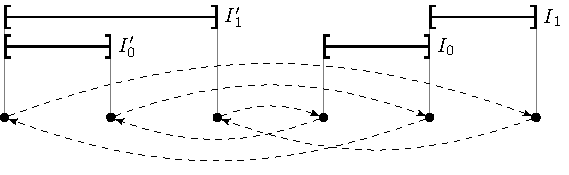
\includegraphics{images/sestcikel.pdf}
% \caption[caption za v kazalo]{Dolg caption pod sliko}
  \caption[Primer vektorske slike.]{Primer 6-cikla.}
  \label{fig:6cikel}
\end{figure}
\end{primer}

\section{Štefanovo zaporedje}
\begin{definicija}
Naj bo $p$ najbolj desna točka intervala $\mathcal{O}$, za katero je $f(p) > p$ in $q\in \mathcal{O}$ prva točka desno od p. Center $c$ cikla $\mathcal{O}$ definiramo kot $c=\frac{p+q}{2}$. Za vsako točko $x \in \mathcal{O}$ označimo množico točk iz cikla $\mathcal{O}$, ki ležijo v zaprtem intervalu omejenem z $x$ in $c$, z $\mathcal{O}_x$. Natančneje, $\mathcal{O}_x = \mathcal{O} \cap [x, p]$, če je $x \leq p$ in  $\mathcal{O}_x = \mathcal{O} \cap [q, x]$, če je $x \geq q$. Pravimo, da točka $x \in \mathcal{O}$ menja strani, če točka $c$ leži med točkama $x$ in $f(x)$.
\end{definicija}

\begin{definicija}
Zaporedje točk $x_0, x_1, \dots, x_n$ je Štefanovo, če:

  \begin{enumerate}[label={(Š\arabic*)}]
    \item $\{x_0, x_1\} = \{p, q\}$, \label{eq:š1}
    \item točke $x_1, x_2, \dots, x_n$ ležijo alternirajoče na levi oziroma desni strani točke $c$. \label{eq:š2}
    \item Zaporedji $x_{2j}$ in $x_{2j+1}$ sta strogo monotoni in se oddaljujeta od točke $c$. \label{eq:š3}
    \item Če je $1\leq j \leq n-1$, potem $x_j$ menja stran in $x_{j+1} \in \mathcal{O}_{f(x_j)}$.\label{eq:š4}
    \item Točka $x_n$ ne menja strani. \label{eq:š5}
  \end{enumerate}
  
\end{definicija}
\begin{opomba}
Štefanofo zaporedje dobimo tako, da iz množice $m$ točk, ki tvorijo $\mathcal{O}$-cikel izberemo $(n+1)$-o točko, ki zadoščajo zgornjim pogojem. 
Pogoj $x_{j+1} \in \mathcal{O}_{f(x_j)}$ v~\ref{eq:š4} pomeni, da je točka $x_{j+1}$ bližje centru kot slika $f(x_j)$ točke $x_j$. Velja ena od neenakosti: $c < x_{j+1} \leq f(x_j)$ ali $f(x_j) \leq x_{j+1} < c$. 
Pogoja~\ref{eq:š2} in~\ref{eq:š3} zagotavljata, da so točke $x_0, x_1, \dots, x_n$ paroma različne. Ker pa lahko pri izbiri točk iz $\mathcal{O}$-cikla tudi kakšno točko izpustimo, je število $n+1$ izbranih točk manjše ali enako številu vseh točk v $\mathcal{O}$-ciklu. Če se vrnemo na primere iz prejšnjega poglavja, lahko vidimo, da v primerih~\ref{primer1}, \ref{primer2} in \ref{primer4} Štefanovo zaporedje sestavljajo vse točke $\mathcal{O}$-cikla. V primeru~\ref{primer3} pa smo dve točki $\mathcal{O}$-cikla ne nastopata v Štefanovem zaporedju.
 Na slikiIz pogoja~\ref{eq:š2} lahko razberemo, da so točke $x_0, x_1, \dots, x_n$ paroma različne. Torej je $n+1 \leq m$ in zato $n<m$. Sliki~\ref{fig:7cikel}
\end{opomba}

\begin{trditev}\label{trd:zap-cikel}
Predpostavimo, da $m$-cikel $\mathcal{O}$ vsebuje Štefanovo zaporedje. Če je $l \triangleleft m$, potem funkcija $f$ vsebuje $\mathcal{O}$-vsiljeno elementarno $l$-zanko $\mathcal{O}$-intervalov in posledično tudi periodično točko z najmanjšo periodo $l$.
\end{trditev}

Pri danem Štefanovem zaporedju $x_0, x_1, \dots, x_n$ definiramo intervale $I_0, I_1, \dots, I_{n-1}$ na  nasledni način: Za $1 \leq j < n$, označimo z $I_j$ najkrajši $\mathcal{O}$-interval, ki vsebuje točke $x_0$, $x_1$ in $x_j$, medtem ko z $I_0$ označimo $\mathcal{O}$-interval s krajišči $x_{n-2}$ in $x_n$. Iz lastnosti~\ref{eq:š2} lahko sklepamo, da je $\interior(I_0) \cap I_j = \emptyset$ za vsak $j \in \{1, 2, \dots, n-1\}$.

\begin{trditev}\label{trd:pokritja}
Za intervale izbrane na zgoraj opisan način veljajo naslednje relacije pokritja:
\begin{enumerate}
\item $I_1 \to I_1$ in $I_0 \to I_1$,\label{trd:pokritja1}
\item $I_1 \to I_2 \to \cdots \to I_{n-1} \to I_0$,\label{trd:pokritja3}
\item $I_0 \to I_{n-1}, I_{n-3}, I_{n-5} \dots $.\label{trd:pokritja2}
\end{enumerate}
Zaradi boljše predstave ponazorimo relacije pokritja na sliki~\ref{fig:nkotnik}.
\end{trditev}

\begin{figure}[h]
  \centering
  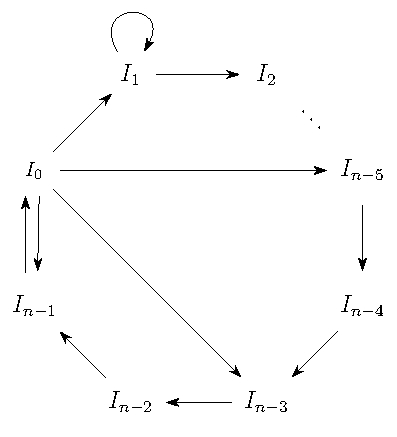
\includegraphics{images/graph_n.pdf}
% \caption[caption za v kazalo]{Dolg caption pod sliko}
  \caption[Primer vektorske slike.]{Primer vektorske slike z oznakami v enaki pisavi, kot jo
     uporablja \LaTeX{}.  Narejena je s programom Inkscape, \LaTeX{} oznake so importane v
     Inkscape iz pomožnega PDF.}
  \label{fig:nkotnik}
\end{figure}

\begin{proof}[Dokaz trditve~\ref{trd:pokritja}]
Dokazovali bomo vsako točko posebej. 

Pri dokazu točke~\ref{trd:pokritja1} bomo dokazali še močnejšo trditev, ki nam bo v pomoč tudi pri dokazu druge točke. Pokazali bomo, da za vsak $j = 0, 1, \dots, n-1$ velja relacija pokritja $I_j \to I_1$.  Za dokaz je dovolj, če se prepričamo, da vsak interval $f(I_j)$ vsebuje točki $x_0$ in $x_1$. V primeru intervala $I_0 = [x_n, x_{n-2}]$ ugotovimo, da obe krajišči $I_0$ ležita na isti strani točke $c$. Lastnost \ref{eq:š4} pove, da krajišče $x_{n-2}$ menja stran, medtem ko lastnost~\ref{eq:š5} pravi, da točka $x_n$ ne menja strani, zato točki $f(x_n)$ in $f(x_{n-2})$ ležita na nasprotnih straneh točke $c$. V primeru intervala $I_j$ za $j = 1, 2, \dots, n-1$ upoštevamo lastnost~\ref{eq:š2} in pridemo do zaključka, da krajišči intervala ležita na nasprotnih straneh točke $c$. Lastnost~\ref{eq:š4} pove, da obe krajišči menjata stran. Torej za vsak $j=0, 1, \dots, n-1$ interval $f(I_j)$ vsebuje točke $\mathcal{O}$-cikla, ki ležijo na obeh straneh centra $c$. Zagotovo vsebuje točki $x_0$ in $x_1$ in zato tudi interval $I_1$.

Naj bo $j$ tako naravno število, za katerega velja $1 \leq j \leq n-1$. Interval $J$ vsebuje interval $I_j$ natanko tedaj, ko vsebuje točke $x_0, x_1$ in $x_j$. Želimo pokazati, da interval $f(x_j)$ vsebuje interval $I_{j+1}$. Vemo že, da interval $f(I_j)$ vsebuje točki $x_0$ in $x_1$. Za dokaz točke~\ref{trd:pokritja2} moramo pokazati samo še vsebovanost točke $x_{j+1}$ v intervalu $f(I_j)$.

Za dokaz točke~\ref{trd:pokritja3} moramo pokazati, da interval $f(I_0)$ vsebuje intervale $I_{n-1}, I_{n-3}, \dots$ Ker že vemo, da $f(I_0)$ vsebuje točki $x_0$ in $x_1$, preostane za dokazati še, da vsebuje točke $x_{n-1}, x_{n-3}, \dots$ Zaradi lastnosti~\ref{eq:š2} ležijo vse točke na drugi strani točke $c$ kot točki $x_{n-2}$ in $x_n$. Iz lastnoti~\ref{eq:š3} sklepamo, da je točka $x_{n-1}$ najbolj oddaljena od točke $c$, zato vsak interval, ki vsebuje točke $x_0, x_1$ in $x_{n-1}$, vsebuje tudi vse točke $x_{n-3}, x_{n-5}, \dots$ Pokazati moramo samo še, da interval $f(I_0$ vsebuje točko $x_{n-1}$. Pri lastnosti~\ref{eq:š4} namesto $j$ pišemo $n-2$ in dobimo vsebovanost $x_{n-1} \in \mathcal{O}_{f(x_j)}$.

\end{proof}


\begin{proof}[Dokaz trditve~\ref{trd:zap-cikel}]
dokaz...
\end{proof}

%#############  KONSTRUKCIJA ŠTEFANOVEGA ZAPOREDJA ##############
\section{Konstrukcija Štefanovega zaporedja}
\begin{trditev}
Cikel, ki vsebuje vsaj eno točko, vsebuje Štefanovo zaporedje, razen če vsaka točka menja stran.
\end{trditev}

 %#############  DOKAZ IZREKA ŠARKOVSKEGA ##############
\section{Dokaz izreka Šarkovskega}

%#############  REALIZACIJSKI IZREK ŠARKOVSKEGA ##############
\section{Realizacijski izrek Šarkovskega}

%#############  IZREK ŠARKOVSKEGA Z ##############
\section{Prostor sharkovskega}

%#############  IZREK ŠARKOVSKEGA Z ##############
\section{Linearni kontinuum je prostor šarkovskega}






% Literatura:
% Primer navajanja na http://www.fmf.uni-lj.si/storage/24240/LiteraturaM.pdf,
% ampak bi moral stil poskrbeti za vse. Reference se uredijo po abecedi.
% Če nobena izbira izmed @book, @atricle,... ni ok, potem se lahko vse napiše v
% @misc pod note={} in deluje tako kot normalen LaTeX.
% Komentar v bib datoteki se naredi samo s parom { }
% Za urejanje literature avtor priporoča program Jabref, ki zna tudi avtomatsko
% okrajšati imena revij. Za pravilno sortiranje vnosov brez avtorja, uporabite
% polje key={ }, kot v primeru.
% V primeru napak ustvarite issue na GitHubu ali pišite na jure.slak@fmf.uni-lj.si.
\cleardoublepage                           % na desni strani
\phantomsection                            % da prav delujejo hiperlinki
\addcontentsline{toc}{section}{\bibname}   % dodajmo v kazalo
\bibliographystyle{fmf-sl}                 % uporabljen stil je v datoteki fmf-sl.bst, na voljo tudi angleška verzija
%\bibliography{\literatura}                 % literatura je v datoteki, definirani na začetku
% TeXStudio zmede \ zgoraj, tako da lahko notri napišeš dejansko ime .bib datoteke, če ti
% ne delajo predlogi citatov.

% Za stvarno kazalo
\cleardoublepage                           % na desni strani
\phantomsection                            % da prav delujejo hiperlinki
\addcontentsline{toc}{section}{\indexname} % dodajmo v kazalo
\printindex

\end{document}


